\documentclass[12pt]{article}
\usepackage[canadien]{babel} 
\usepackage[utf8]{inputenc}
\usepackage[T1]{fontenc}
\usepackage{fancyhdr}
\usepackage{graphicx}
\usepackage{enumerate}
\usepackage{amsmath}
\usepackage{amssymb}
\usepackage{subfigure}
\usepackage{amsmath}
\usepackage{amssymb}
\usepackage{bm}
\usepackage{url}
\usepackage[dvipsnames]{xcolor}
\usepackage{todonotes}

% If your paper is accepted, change the options for the package
% aistats2e as follows:
%
%\usepackage[accepted]{aistats2e}
%
% This option will print headings for the title of your paper and
% headings for the authors names, plus a copyright note at the end of
% the first column of the first page.
\setlength{\parindent}{0cm}
\addtolength{\oddsidemargin}{-2cm}
\addtolength{\evensidemargin}{-2cm}
\setlength{\textwidth}{17.78cm}
\addtolength{\topmargin}{-2.25cm}
\setlength{\textheight}{23.24cm}
\addtolength{\parskip}{5mm}
\pagestyle{fancy}

%************
%* COMMANDS *
%************

%%%%% NEW MATH DEFINITIONS %%%%%

% Mark sections of captions for referring to divisions of figures
\newcommand{\figleft}{{\em (Left)}}
\newcommand{\figcenter}{{\em (Center)}}
\newcommand{\figright}{{\em (Right)}}
\newcommand{\figtop}{{\em (Top)}}
\newcommand{\figbottom}{{\em (Bottom)}}
\newcommand{\captiona}{{\em (a)}}
\newcommand{\captionb}{{\em (b)}}
\newcommand{\captionc}{{\em (c)}}
\newcommand{\captiond}{{\em (d)}}

% Highlight a newly defined term
\newcommand{\newterm}[1]{{\bf #1}}


% Figure reference, lower-case.
\def\figref#1{figure~\ref{#1}}
% Figure reference, capital. For start of sentence
\def\Figref#1{Figure~\ref{#1}}
\def\twofigref#1#2{figures \ref{#1} and \ref{#2}}
\def\quadfigref#1#2#3#4{figures \ref{#1}, \ref{#2}, \ref{#3} and \ref{#4}}
% Section reference, lower-case.
\def\secref#1{section~\ref{#1}}
% Section reference, capital.
\def\Secref#1{Section~\ref{#1}}
% Reference to two sections.
\def\twosecrefs#1#2{sections \ref{#1} and \ref{#2}}
% Reference to three sections.
\def\secrefs#1#2#3{sections \ref{#1}, \ref{#2} and \ref{#3}}
% Reference to an equation, lower-case.
\def\eqref#1{equation~\ref{#1}}
% Reference to an equation, upper case
\def\Eqref#1{Equation~\ref{#1}}
% A raw reference to an equation---avoid using if possible
\def\plaineqref#1{\ref{#1}}
% Reference to a chapter, lower-case.
\def\chapref#1{chapter~\ref{#1}}
% Reference to an equation, upper case.
\def\Chapref#1{Chapter~\ref{#1}}
% Reference to a range of chapters
\def\rangechapref#1#2{chapters\ref{#1}--\ref{#2}}
% Reference to an algorithm, lower-case.
\def\algref#1{algorithm~\ref{#1}}
% Reference to an algorithm, upper case.
\def\Algref#1{Algorithm~\ref{#1}}
\def\twoalgref#1#2{algorithms \ref{#1} and \ref{#2}}
\def\Twoalgref#1#2{Algorithms \ref{#1} and \ref{#2}}
% Reference to a part, lower case
\def\partref#1{part~\ref{#1}}
% Reference to a part, upper case
\def\Partref#1{Part~\ref{#1}}
\def\twopartref#1#2{parts \ref{#1} and \ref{#2}}

\def\ceil#1{\lceil #1 \rceil}
\def\floor#1{\lfloor #1 \rfloor}
\def\1{\bm{1}}
\newcommand{\train}{\mathcal{D}}
\newcommand{\valid}{\mathcal{D_{\mathrm{valid}}}}
\newcommand{\test}{\mathcal{D_{\mathrm{test}}}}

\def\eps{{\epsilon}}


% Random variables
\def\reta{{\textnormal{$\eta$}}}
\def\ra{{\textnormal{a}}}
\def\rb{{\textnormal{b}}}
\def\rc{{\textnormal{c}}}
\def\rd{{\textnormal{d}}}
\def\re{{\textnormal{e}}}
\def\rf{{\textnormal{f}}}
\def\rg{{\textnormal{g}}}
\def\rh{{\textnormal{h}}}
\def\ri{{\textnormal{i}}}
\def\rj{{\textnormal{j}}}
\def\rk{{\textnormal{k}}}
\def\rl{{\textnormal{l}}}
% rm is already a command, just don't name any random variables m
\def\rn{{\textnormal{n}}}
\def\ro{{\textnormal{o}}}
\def\rp{{\textnormal{p}}}
\def\rq{{\textnormal{q}}}
\def\rr{{\textnormal{r}}}
\def\rs{{\textnormal{s}}}
\def\rt{{\textnormal{t}}}
\def\ru{{\textnormal{u}}}
\def\rv{{\textnormal{v}}}
\def\rw{{\textnormal{w}}}
\def\rx{{\textnormal{x}}}
\def\ry{{\textnormal{y}}}
\def\rz{{\textnormal{z}}}

% Random vectors
\def\rvepsilon{{\mathbf{\epsilon}}}
\def\rvtheta{{\mathbf{\theta}}}
\def\rva{{\mathbf{a}}}
\def\rvb{{\mathbf{b}}}
\def\rvc{{\mathbf{c}}}
\def\rvd{{\mathbf{d}}}
\def\rve{{\mathbf{e}}}
\def\rvf{{\mathbf{f}}}
\def\rvg{{\mathbf{g}}}
\def\rvh{{\mathbf{h}}}
\def\rvu{{\mathbf{i}}}
\def\rvj{{\mathbf{j}}}
\def\rvk{{\mathbf{k}}}
\def\rvl{{\mathbf{l}}}
\def\rvm{{\mathbf{m}}}
\def\rvn{{\mathbf{n}}}
\def\rvo{{\mathbf{o}}}
\def\rvp{{\mathbf{p}}}
\def\rvq{{\mathbf{q}}}
\def\rvr{{\mathbf{r}}}
\def\rvs{{\mathbf{s}}}
\def\rvt{{\mathbf{t}}}
\def\rvu{{\mathbf{u}}}
\def\rvv{{\mathbf{v}}}
\def\rvw{{\mathbf{w}}}
\def\rvx{{\mathbf{x}}}
\def\rvy{{\mathbf{y}}}
\def\rvz{{\mathbf{z}}}

% Elements of random vectors
\def\erva{{\textnormal{a}}}
\def\ervb{{\textnormal{b}}}
\def\ervc{{\textnormal{c}}}
\def\ervd{{\textnormal{d}}}
\def\erve{{\textnormal{e}}}
\def\ervf{{\textnormal{f}}}
\def\ervg{{\textnormal{g}}}
\def\ervh{{\textnormal{h}}}
\def\ervi{{\textnormal{i}}}
\def\ervj{{\textnormal{j}}}
\def\ervk{{\textnormal{k}}}
\def\ervl{{\textnormal{l}}}
\def\ervm{{\textnormal{m}}}
\def\ervn{{\textnormal{n}}}
\def\ervo{{\textnormal{o}}}
\def\ervp{{\textnormal{p}}}
\def\ervq{{\textnormal{q}}}
\def\ervr{{\textnormal{r}}}
\def\ervs{{\textnormal{s}}}
\def\ervt{{\textnormal{t}}}
\def\ervu{{\textnormal{u}}}
\def\ervv{{\textnormal{v}}}
\def\ervw{{\textnormal{w}}}
\def\ervx{{\textnormal{x}}}
\def\ervy{{\textnormal{y}}}
\def\ervz{{\textnormal{z}}}

% Random matrices
\def\rmA{{\mathbf{A}}}
\def\rmB{{\mathbf{B}}}
\def\rmC{{\mathbf{C}}}
\def\rmD{{\mathbf{D}}}
\def\rmE{{\mathbf{E}}}
\def\rmF{{\mathbf{F}}}
\def\rmG{{\mathbf{G}}}
\def\rmH{{\mathbf{H}}}
\def\rmI{{\mathbf{I}}}
\def\rmJ{{\mathbf{J}}}
\def\rmK{{\mathbf{K}}}
\def\rmL{{\mathbf{L}}}
\def\rmM{{\mathbf{M}}}
\def\rmN{{\mathbf{N}}}
\def\rmO{{\mathbf{O}}}
\def\rmP{{\mathbf{P}}}
\def\rmQ{{\mathbf{Q}}}
\def\rmR{{\mathbf{R}}}
\def\rmS{{\mathbf{S}}}
\def\rmT{{\mathbf{T}}}
\def\rmU{{\mathbf{U}}}
\def\rmV{{\mathbf{V}}}
\def\rmW{{\mathbf{W}}}
\def\rmX{{\mathbf{X}}}
\def\rmY{{\mathbf{Y}}}
\def\rmZ{{\mathbf{Z}}}

% Elements of random matrices
\def\ermA{{\textnormal{A}}}
\def\ermB{{\textnormal{B}}}
\def\ermC{{\textnormal{C}}}
\def\ermD{{\textnormal{D}}}
\def\ermE{{\textnormal{E}}}
\def\ermF{{\textnormal{F}}}
\def\ermG{{\textnormal{G}}}
\def\ermH{{\textnormal{H}}}
\def\ermI{{\textnormal{I}}}
\def\ermJ{{\textnormal{J}}}
\def\ermK{{\textnormal{K}}}
\def\ermL{{\textnormal{L}}}
\def\ermM{{\textnormal{M}}}
\def\ermN{{\textnormal{N}}}
\def\ermO{{\textnormal{O}}}
\def\ermP{{\textnormal{P}}}
\def\ermQ{{\textnormal{Q}}}
\def\ermR{{\textnormal{R}}}
\def\ermS{{\textnormal{S}}}
\def\ermT{{\textnormal{T}}}
\def\ermU{{\textnormal{U}}}
\def\ermV{{\textnormal{V}}}
\def\ermW{{\textnormal{W}}}
\def\ermX{{\textnormal{X}}}
\def\ermY{{\textnormal{Y}}}
\def\ermZ{{\textnormal{Z}}}

% Vectors
\def\vzero{{\bm{0}}}
\def\vone{{\bm{1}}}
\def\vmu{{\bm{\mu}}}
\def\vtheta{{\bm{\theta}}}
\def\va{{\bm{a}}}
\def\vb{{\bm{b}}}
\def\vc{{\bm{c}}}
\def\vd{{\bm{d}}}
\def\ve{{\bm{e}}}
\def\vf{{\bm{f}}}
\def\vg{{\bm{g}}}
\def\vh{{\bm{h}}}
\def\vi{{\bm{i}}}
\def\vj{{\bm{j}}}
\def\vk{{\bm{k}}}
\def\vl{{\bm{l}}}
\def\vm{{\bm{m}}}
\def\vn{{\bm{n}}}
\def\vo{{\bm{o}}}
\def\vp{{\bm{p}}}
\def\vq{{\bm{q}}}
\def\vr{{\bm{r}}}
\def\vs{{\bm{s}}}
\def\vt{{\bm{t}}}
\def\vu{{\bm{u}}}
\def\vv{{\bm{v}}}
\def\vw{{\bm{w}}}
\def\vx{{\bm{x}}}
\def\vy{{\bm{y}}}
\def\vz{{\bm{z}}}

% Elements of vectors
\def\evalpha{{\alpha}}
\def\evbeta{{\beta}}
\def\evepsilon{{\epsilon}}
\def\evlambda{{\lambda}}
\def\evomega{{\omega}}
\def\evmu{{\mu}}
\def\evpsi{{\psi}}
\def\evsigma{{\sigma}}
\def\evtheta{{\theta}}
\def\eva{{a}}
\def\evb{{b}}
\def\evc{{c}}
\def\evd{{d}}
\def\eve{{e}}
\def\evf{{f}}
\def\evg{{g}}
\def\evh{{h}}
\def\evi{{i}}
\def\evj{{j}}
\def\evk{{k}}
\def\evl{{l}}
\def\evm{{m}}
\def\evn{{n}}
\def\evo{{o}}
\def\evp{{p}}
\def\evq{{q}}
\def\evr{{r}}
\def\evs{{s}}
\def\evt{{t}}
\def\evu{{u}}
\def\evv{{v}}
\def\evw{{w}}
\def\evx{{x}}
\def\evy{{y}}
\def\evz{{z}}

% Matrix
\def\mA{{\bm{A}}}
\def\mB{{\bm{B}}}
\def\mC{{\bm{C}}}
\def\mD{{\bm{D}}}
\def\mE{{\bm{E}}}
\def\mF{{\bm{F}}}
\def\mG{{\bm{G}}}
\def\mH{{\bm{\text{\textbf{H}}}}}
\def\mI{{\bm{I}}}
\def\mJ{{\bm{J}}}
\def\mK{{\bm{K}}}
\def\mL{{\bm{L}}}
\def\mM{{\bm{M}}}
\def\mN{{\bm{N}}}
\def\mO{{\bm{O}}}
\def\mP{{\bm{P}}}
\def\mQ{{\bm{Q}}}
\def\mR{{\bm{R}}}
\def\mS{{\bm{S}}}
\def\mT{{\bm{T}}}
\def\mU{{\bm{U}}}
\def\mV{{\bm{V}}}
\def\mW{{\bm{W}}}
\def\mX{{\bm{X}}}
\def\mY{{\bm{Y}}}
\def\mZ{{\bm{Z}}}
\def\mBeta{{\bm{\beta}}}
\def\mPhi{{\bm{\Phi}}}
\def\mLambda{{\bm{\Lambda}}}
\def\mSigma{{\bm{\Sigma}}}

% Tensor
\DeclareMathAlphabet{\mathsfit}{\encodingdefault}{\sfdefault}{m}{sl}
\SetMathAlphabet{\mathsfit}{bold}{\encodingdefault}{\sfdefault}{bx}{n}
\newcommand{\tens}[1]{\bm{\mathsfit{#1}}}
\def\tA{{\tens{A}}}
\def\tB{{\tens{B}}}
\def\tC{{\tens{C}}}
\def\tD{{\tens{D}}}
\def\tE{{\tens{E}}}
\def\tF{{\tens{F}}}
\def\tG{{\tens{G}}}
\def\tH{{\tens{H}}}
\def\tI{{\tens{I}}}
\def\tJ{{\tens{J}}}
\def\tK{{\tens{K}}}
\def\tL{{\tens{L}}}
\def\tM{{\tens{M}}}
\def\tN{{\tens{N}}}
\def\tO{{\tens{O}}}
\def\tP{{\tens{P}}}
\def\tQ{{\tens{Q}}}
\def\tR{{\tens{R}}}
\def\tS{{\tens{S}}}
\def\tT{{\tens{T}}}
\def\tU{{\tens{U}}}
\def\tV{{\tens{V}}}
\def\tW{{\tens{W}}}
\def\tX{{\tens{X}}}
\def\tY{{\tens{Y}}}
\def\tZ{{\tens{Z}}}


% Graph
\def\gA{{\mathcal{A}}}
\def\gB{{\mathcal{B}}}
\def\gC{{\mathcal{C}}}
\def\gD{{\mathcal{D}}}
\def\gE{{\mathcal{E}}}
\def\gF{{\mathcal{F}}}
\def\gG{{\mathcal{G}}}
\def\gH{{\mathcal{H}}}
\def\gI{{\mathcal{I}}}
\def\gJ{{\mathcal{J}}}
\def\gK{{\mathcal{K}}}
\def\gL{{\mathcal{L}}}
\def\gM{{\mathcal{M}}}
\def\gN{{\mathcal{N}}}
\def\gO{{\mathcal{O}}}
\def\gP{{\mathcal{P}}}
\def\gQ{{\mathcal{Q}}}
\def\gR{{\mathcal{R}}}
\def\gS{{\mathcal{S}}}
\def\gT{{\mathcal{T}}}
\def\gU{{\mathcal{U}}}
\def\gV{{\mathcal{V}}}
\def\gW{{\mathcal{W}}}
\def\gX{{\mathcal{X}}}
\def\gY{{\mathcal{Y}}}
\def\gZ{{\mathcal{Z}}}

% Sets
\def\sA{{\mathbb{A}}}
\def\sB{{\mathbb{B}}}
\def\sC{{\mathbb{C}}}
\def\sD{{\mathbb{D}}}
% Don't use a set called E, because this would be the same as our symbol
% for expectation.
\def\sF{{\mathbb{F}}}
\def\sG{{\mathbb{G}}}
\def\sH{{\mathbb{H}}}
\def\sI{{\mathbb{I}}}
\def\sJ{{\mathbb{J}}}
\def\sK{{\mathbb{K}}}
\def\sL{{\mathbb{L}}}
\def\sM{{\mathbb{M}}}
\def\sN{{\mathbb{N}}}
\def\sO{{\mathbb{O}}}
\def\sP{{\mathbb{P}}}
\def\sQ{{\mathbb{Q}}}
\def\sR{{\mathbb{R}}}
\def\sS{{\mathbb{S}}}
\def\sT{{\mathbb{T}}}
\def\sU{{\mathbb{U}}}
\def\sV{{\mathbb{V}}}
\def\sW{{\mathbb{W}}}
\def\sX{{\mathbb{X}}}
\def\sY{{\mathbb{Y}}}
\def\sZ{{\mathbb{Z}}}

% Entries of a matrix
\def\emLambda{{\Lambda}}
\def\emA{{A}}
\def\emB{{B}}
\def\emC{{C}}
\def\emD{{D}}
\def\emE{{E}}
\def\emF{{F}}
\def\emG{{G}}
\def\emH{{H}}
\def\emI{{I}}
\def\emJ{{J}}
\def\emK{{K}}
\def\emL{{L}}
\def\emM{{M}}
\def\emN{{N}}
\def\emO{{O}}
\def\emP{{P}}
\def\emQ{{Q}}
\def\emR{{R}}
\def\emS{{S}}
\def\emT{{T}}
\def\emU{{U}}
\def\emV{{V}}
\def\emW{{W}}
\def\emX{{X}}
\def\emY{{Y}}
\def\emZ{{Z}}
\def\emSigma{{\Sigma}}

% entries of a tensor
% Same font as tensor, without \bm wrapper
\newcommand{\etens}[1]{\mathsfit{#1}}
\def\etLambda{{\etens{\Lambda}}}
\def\etA{{\etens{A}}}
\def\etB{{\etens{B}}}
\def\etC{{\etens{C}}}
\def\etD{{\etens{D}}}
\def\etE{{\etens{E}}}
\def\etF{{\etens{F}}}
\def\etG{{\etens{G}}}
\def\etH{{\etens{H}}}
\def\etI{{\etens{I}}}
\def\etJ{{\etens{J}}}
\def\etK{{\etens{K}}}
\def\etL{{\etens{L}}}
\def\etM{{\etens{M}}}
\def\etN{{\etens{N}}}
\def\etO{{\etens{O}}}
\def\etP{{\etens{P}}}
\def\etQ{{\etens{Q}}}
\def\etR{{\etens{R}}}
\def\etS{{\etens{S}}}
\def\etT{{\etens{T}}}
\def\etU{{\etens{U}}}
\def\etV{{\etens{V}}}
\def\etW{{\etens{W}}}
\def\etX{{\etens{X}}}
\def\etY{{\etens{Y}}}
\def\etZ{{\etens{Z}}}

% The true underlying data generating distribution
\newcommand{\pdata}{p_{\rm{data}}}
% The empirical distribution defined by the training set
\newcommand{\ptrain}{\hat{p}_{\rm{data}}}
\newcommand{\Ptrain}{\hat{P}_{\rm{data}}}
% The model distribution
\newcommand{\pmodel}{p_{\rm{model}}}
\newcommand{\Pmodel}{P_{\rm{model}}}
\newcommand{\ptildemodel}{\tilde{p}_{\rm{model}}}
% Stochastic autoencoder distributions
\newcommand{\pencode}{p_{\rm{encoder}}}
\newcommand{\pdecode}{p_{\rm{decoder}}}
\newcommand{\precons}{p_{\rm{reconstruct}}}

\newcommand{\laplace}{\mathrm{Laplace}} % Laplace distribution

\newcommand{\E}{\mathbb{E}}
\newcommand{\Ls}{\mathcal{L}}
\newcommand{\R}{\mathbb{R}}
\newcommand{\emp}{\tilde{p}}
\newcommand{\lr}{\alpha}
\newcommand{\reg}{\lambda}
\newcommand{\rect}{\mathrm{rectifier}}
\newcommand{\softmax}{\mathrm{softmax}}
\newcommand{\sigmoid}{\sigma}
\newcommand{\softplus}{\zeta}
\newcommand{\KL}{D_{\mathrm{KL}}}
\newcommand{\Var}{\mathrm{Var}}
\newcommand{\standarderror}{\mathrm{SE}}
\newcommand{\Cov}{\mathrm{Cov}}
% Wolfram Mathworld says $L^2$ is for function spaces and $\ell^2$ is for vectors
% But then they seem to use $L^2$ for vectors throughout the site, and so does
% wikipedia.
\newcommand{\normlzero}{L^0}
\newcommand{\normlone}{L^1}
\newcommand{\normltwo}{L^2}
\newcommand{\normlp}{L^p}
\newcommand{\normmax}{L^\infty}

\newcommand{\parents}{Pa} % See usage in notation.tex. Chosen to match Daphne's book.

\DeclareMathOperator*{\argmax}{arg\,max}
\DeclareMathOperator*{\argmin}{arg\,min}

\DeclareMathOperator{\sign}{sign}
\DeclareMathOperator{\Tr}{Tr}
\let\ab\allowbreak


%%% new
\newcommand{\diag}{\mathop{\mathrm{diag}}\nolimits}
\usepackage{cancel}
\newcommand{\ttt}[1]{\texttt{#1}}

\newif\ifexercise
\exercisetrue
%\exercisefalse

\newif\ifsolution
\solutiontrue
%\solutionfalse

\usepackage{booktabs}
\usepackage[ruled,vlined]{algorithm2e}

\usepackage{amsthm}
\theoremstyle{definition}
\newtheorem{exercise}{Question}%[chapter]
\newtheorem{answer}{Answer} % asterisk to remove ordering

\newcommand{\Exercise}[1]{
\ifexercise#1\fi
}


\definecolor{answer}{rgb}{0.00, 0.12, 0.60}
\newcommand{\Answer}[1]{
\ifsolution\color{answer}\begin{answer}#1\end{answer}\fi
}

\newif\ifexercise
\exercisetrue
%\exercisefalse

\newif\ifsolution
\solutiontrue
%\solutionfalse

\newcommand{\pder}[2]{\frac{\partial #1}{\partial #2}}
\usepackage{enumitem}
\newcommand{\staritem}{
\addtocounter{enumi}{1}
\item[$\phantom{x}^{*}$\theenumi]}
\setlist[enumerate,1]{leftmargin=*, label=\arabic*.}

\begin{document}


\fancyhead{}
\fancyfoot{}

\fancyhead[L]{
  \begin{tabular}[b]{l}
    IFT6135-A2023  \\
    Prof: Aishwarya Agrawal \\
  \end{tabular}
}
\fancyhead[R]{
  \begin{tabular}[b]{r}
    Assignment 1  \\
    Multilayer Perceptrons and Convolutional Neural Networks \\
  \end{tabular}
}
\fancyfoot[C]{- Do not distribute -}

\vspace{1cm}

\shorthandoff{:}
{\textbf{Due Date: October 19th, 2023 at 11:00 pm}}\\


\vspace{-0.5cm}
\underline{Instructions}%
\renewcommand{\labelitemi}{\textbullet}

\begin{itemize}
\item \emph{For all questions, show your work!}
\item \emph{Use LaTeX and the template we provide when writing your answers.
You may reuse most of the notation shorthands, equations and/or tables.
See the assignment policy on the course website for more details.}
\item \emph{The use of AI tools like Chat-GPT to find answers or parts of answers for any question in this assignment is not allowed. However, you can use these tools to improve the quality of your writing, like fixing grammar or making it more understandable. If you do use these tools, you must clearly explain how you used them and which questions or parts of questions you applied them to. Failing to do so or using these tools to find answers or parts of answers may result in your work being completely rejected, which means you'll receive a score of 0 for the entire theory or practical section.}
\item \emph{Submit your answers electronically via Gradescope.}
\item \emph{TAs for this assignment are \textbf{Saba Ahmadi, Sahar Dastani, and Sophie Xhonneux.}}
\end{itemize}

\vspace{0.2cm}

% Q1
\begin{exercise}[5-2-2-1-3-2] (\textbf{Activation Functions and Backpropagation})
\Exercise{
\label{ex:activation}
\emph{Please note that during marking we will not read more than the question says you should write, e.g.\ if the question asks for one sentence, only the first sentence will be read.}
\begin{enumerate}
    \item Given the following 3 layer neural network $\vo = f(\vx)$
    \begin{equation}
    \begin{aligned}
        \vh &= \mW_1 \vx + \vb_1 \\
        \va &= \sigmoid( \mW_2 \vh + \vb_2 ) \\
        \vo &= \mW_3 \va +\vb_3,
    \end{aligned}
    \end{equation}
    where $\vx\in\mathrm{R}^n$, $\vh\in\mathrm{R}^m$, $\va\in\mathrm{R}^r$, $\vo\in\mathrm{R}^s$, $\sigmoid(x) = \frac{1}{1+e^{-x}}$, and a loss function $\mathrm{L}(\vo,\vy)$ apply the backpropagation algorithm computing the gradients with respect to the weights $\mW_1,\mW_2,\mW_3, \vb_1,\vb_2,\vb_3$ to show which are the necessary intermediate vectors that we need to store during the forward pass such as to not need recomputation. Use the notation provided above.
    \item Assuming each floating point number takes two bytes to store, give the amount of memory in bytes, needed to store during the forward pass for the backward pass to not need recomputation.
    \item Compute the left and right derivative of the \texttt{ReLU} function at $x=0$. Show your work.
    \item Give \textbf{one} sentence to explain why we cannot use the \texttt{ReLU} function if we want to differentiate our neural network twice.
    \item The swish activation function is defined as $ g(x) = x  \sigmoid(\beta  x)$. Simplify the function in the limit as $\beta$ approaches 0 and infinity. Show your work.
    \item Give 1 reason (one sentence) as to why we might want to use the swish function over the \texttt{ReLU}. Give 1 reason (one sentence) as to why we might want to use the \texttt{ReLU} over the swish (hint: monotonicity).
\end{enumerate}
}

\Answer{
% Write your answer here
% TODO: add z and \sigma in calculations...
\subsubsection*{1}
Let $z=W_{2}h+b_{2}$.
  \begin{align*}
    \pder{L}{W_1} &= \pder{L}{o} \pder{o}{a} \pder{a}{\sigma} \pder{\sigma}{z}\pder{z}{h}\pder{h}{W_{1}}\\
    &= \pder{L}{o} W_{3} \sigma(a)(\bold{1}-\sigma(W_{2}h+b_{2}))W_{2}x^{T}\\
    &= \pder{L}{o} W_{3} (\bold{1}-a) W_{2} x^{T}
  \end{align*}
  To calculate the gradient with respect to $W_{1}$, we need to store the
  vectors $x,\, a $ and the matrix and $W_{3}$
  \begin{align*}
    \pder{L}{W_2} &= \pder{L}{o}\pder{o}{a} \pder{a}{\sigma} \pder{\sigma}{W_{2}} \\
    &= \pder{L}{o}  W_{3} (\bold{1}-\sigma(W_{2}h+b_{2}))h^{T}\\
    &= \pder{L}{o} W_{3} (\bold{1}-a) h^{T}
  \end{align*}
  To calculate the gradient with respect to $W_{2}$, we need to store the
  vectors $ h,\, a $ and the matrix and $W_{3}$
  \begin{align*}
    \pder{L}{W_3} &= \pder{L}{o}\pder{o}{W_{3}} \\
    &= \pder{L}{o}a^{T}
  \end{align*}
  To calculate the gradient with respect to $W_{3}$, we need to store the
  vector $a$.
  \begin{align*}
    \pder{L}{b_{1}} &=   \pder{h}{b_{1}}\pder{\sigma}{h}\pder{a}{\sigma} \pder{o}{a} \pder{L}{o}\\
    &= (\bold{1}-\sigma(W_{2}h+b_{2})) W_{3} \pder{L}{o}\\
    &= (\bold{1}-a) W_{3} \pder{L}{o}
  \end{align*}
  To calculate the gradient with respect to $b_{1}$, we need to store the
  vectors $ a $ and the matrix $W_{2}$.
  \begin{align*}
    \pder{L}{b_{2}} &=\pder{\sigma}{b_{2}} \pder{a}{\sigma} \pder{o}{a} \pder{L}{o}\\
    &=  (\bold{1}-\sigma(W_{2}h+b_{2})) W_{3} \pder{L}{o}\\
    &=  (\bold{1}-a) W_{3} \pder{L}{o}
  \end{align*}
  To calculate the gradient with respect to $b_{2}$, we need to store the
  vectors $ a $ and the matrix $W_{3}$.
  \begin{align*}
    \pder{L}{b_{3}} &= \pder{o}{b_{3}} \pder{L}{o}\\
    &= \pder{L}{o}
  \end{align*}
  To calculate the gradient with respect to $b_{3}$, we don need to store any
  vector. We only need to compute the derivative of $L$ with respect to $o$.
\subsubsection*{2}
  To compute the gradient with respect to $W_{1}, W_{2}, W_{3}, b_{1}, b_{2}$ and
  $b_{3}$, we need to store the following vectors and matrices:
  \begin{equation*}
    x \in \R^{n}, \, a \in \R^{r}, \, h \in \R^{m}, \,W_{3} \in \R^{s \times r}, \, W_{2} \in \R^{r \times m}.
  \end{equation*}Therefore, we need a total amount of $2(n+r+m+sr+rm)$ bytes to
  store all of these numbers.
\subsubsection*{3}
Firstly, we need to calculate the right limit:
\begin{equation*}
  \lim_{x\to0} \frac{ Relu(x)-0 }{x-0},\, x > 0
\end{equation*}This limit is obvously 1, as the expression can be reduced to 1
because $Relu(x) = x$ when $x\geq0$.
The other left side derivative is

\begin{align*}
  \lim_{x\to0} \frac{ Relu(x)-0 }{x-0} &= \lim_{x\to0} \frac{0}{x} \\
  &= 0 \, \text{for $x$ < 0}
\end{align*}We can conclude that the left side derivative is 0 around 0.

}
\subsubsection*{4}It would make our gradients vanish (i.e. equals 0) as the second derivative of
the $Relu$ function is always $0$.
\subsubsection{5}
The swish function is defined as $g(x) = \frac{x}{1+e^{-\beta x}}$. Let's first
calculate the limit when $\beta \to 0$:
\begin{align*}
  \lim_{\beta \to 0} \frac{x}{1+e^{-\beta x}} &= \frac{x}{1+\lim_{\beta \to 0} e^{-\beta x}}\\
  &=  \frac{x}{1+ e^{\lim_{\beta \to 0}-\beta x}} \quad \text{$e^{x}$ is continuous}\\
  &=  \frac{x}{1+ e^{0}}\\
  &=  \frac{x}{2}
\end{align*}
We can calculate the limit when $\beta \to \infty$:
\begin{align*}
  \lim_{\beta \to \infty} \frac{x}{1+e^{-\beta x}} &= \frac{x}{1+\lim_{\beta \to \infty} e^{-\beta x}}\\
  &= \frac{x}{1+\lim_{\beta \to \infty} \frac{1}{e^{\beta x}}}\\
  &=  \frac{x}{1+ 0}\\
  &=  x
\end{align*}
\subsubsection*{6}
%TODO: Find a real answer
We might prefer the swish function because it is a smooth function. We might
prefer the Relu function because it is convex.
\end{exercise}

% Q2
\begin{exercise}[4-4-5-3] (\textbf{Convolution Basics})
\Exercise{
\label{ex:cnn}
\begin{enumerate}
    \item \textbf{Short answers:}
    \begin{enumerate}
        \item When you apply a filter to feature maps, under what conditions does the size of the feature map decrease?
        \item What impact does a larger stride have?
        \item Explain what you understand from the term "sparse connections" in terms of connections between two layers in a neural network.
        \item As we are aware, each \textit{Convolutional} layer contains learnable parameters, including weights and biases. If you decide not to include biases in the \textit{Convolution} layer of the following network, what will be the impact on its performance (compared to the case when the \textit{Convolution} layer includes biases)?
        $$Input \rightarrow Convolution \rightarrow Batch Norm \rightarrow Activation \rightarrow Output$$
    \end{enumerate}
    \item \textbf{True/False:}
    \begin{enumerate}
        \item In a convolutional layer, the number of weights is contingent upon the depth of the input data volume.
        \item In a convolutional layer, the number of biases equals the number of filters.
        \item The total number of parameters is influenced by the stride and padding.
        \item Maxpooling operates only on the height and width dimensions of an image.
    \end{enumerate}
    \item \textbf{Convolutional Architecture:} Let's analyze the convolutional neural network (CNN) defined by the layers in the left column. For each layer, determine the output volume's shape and the number of parameters. It's worth noting that in our notation, "Conv4-N-Pvalid-S2" represents a convolutional layer with N 4x4 filters, valid padding, and a stride of 2.

    \begin{center}
    \begin{tabular}{| c | c | c |} 
     \hline
     Layers & Output volume dimensions & Number of parameters \\ [0.5ex] 
     \hline
     Input & $64 \times 64 \times 1$ &  \\ 
     \hline
     Conv4-5-Pvalid-S2 &  &  \\
     \hline
     Pool3 &  &  \\
     \hline
     Conv3-5-Pvalid-S1 &  &  \\
     \hline
     Pool2 &  &  \\ [1ex] 
     \hline
     FC5 &  &  \\ [1ex] 
     \hline
    \end{tabular}
    \end{center}
% latexmk -pvc <file>.tex
    \item \textbf{Receptive Fields:} Receptive Field is defined as the size of the region in the input that produces a feature. For example, when using a Conv-3x3 layer, each feature is generated by a 3x3 grid in the input. Having two Conv-3x3 layers in succession leads to a 5x5 receptive field. An example of this is outlined in Figure \ref{fig:Obj-1}. Note that there is a receptive field associated with each feature (Figure \ref{fig:Obj-1} shows the receptive field associated with the yellow-colored feature in Layer 3), where a feature is a cell in the output activation map. 

    \begin{figure}
      \centering
      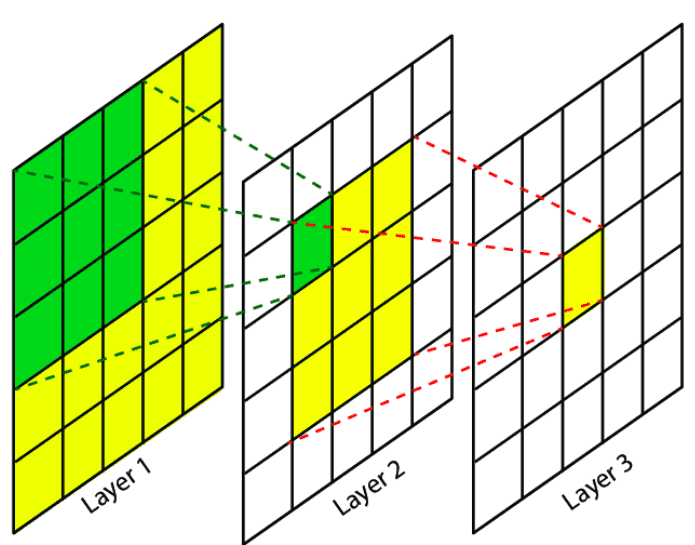
\includegraphics[width=0.25\columnwidth,natwidth=610,natheight=642]{Figures/receptive.png}
      \caption{Illustration of Receptive Field.}
      \label{fig:Obj-1}
    \end{figure}

    Consider a network architecture consisting solely of 5 Convolution layers, each with kernel size 5, stride 1, zero-padding of two pixels on all four sides, 8 intermediate channels, and one output channel. What is the receptive field of the final features obtained through this architecture, that is, what is the size of the input that corresponds to a particular pixel position in the output?
\end{enumerate}
}

\Answer{
% Write your answer here
\subsubsection*{1}
\begin{enumerate}[label=(\alph*)]
 \item If you apply a filter with a receptive field bigger than 1, and without
% TODO
insert padding name here padding, the feature map size decrease.
 \item It reduces the size of the feature map
 \item
% TODO: Better formulation
Two layers are sparsely connected if the matrix $A$ in the  is mostly composed of
zeroes
 \item The bias inside the convolution layer are not useful in this case,
        substracted by the normalization  and then added back by the Batch
        normalization layer.
\end{enumerate}
\subsubsection*{2}
\begin{enumerate}[label=(\alph*)]
\item aka le nombre de channels est important ?
\item False
\item True
\item
\end{enumerate}
\subsubsection*{3}

    \begin{center}
    \begin{tabular}{| c | c | c |}
     \hline
     Layers & Output volume dimensions & Number of parameters \\ [0.5ex]
     \hline
     Input & $64 \times 64 \times 1$ & 0  \\
     \hline
     Conv4-5-Pvalid-S2 & $31 \times 31 \times 5$  & $(4 \times 4 \times 1 + 1) \times 5 = 85$ \\
     \hline
     Pool3 & $29 \times 29 \times 5$ &  0 \\
     \hline
     Conv3-5-Pvalid-S1 & $27 \times 27 \times 5$ & $(3 \times 3 \times 1 + 1) \times 5 = 50$ \\
     \hline
     Pool2 & $26 \times 26 \times 5$ &  0 \\ [1ex]
     \hline
     FC5 & $5 \times 1 \times 1$ & $26 \times (26 +1) \times 5 = 3510$ \\ [1ex]
     \hline
    \end{tabular}
    \end{center}
\subsubsection*{4}
}
\end{exercise}

% Q3
\begin{exercise}[10] (\textbf{Mixture Models meet Neural Networks})
\Exercise{
\label{ex:mixture_model}

Consider modelling some data $\{(\vx_n, y_n)\}_{n=1}^N$, $\vx_n \in \mathbb{R}^d$, $y_n \in \{0,1\}$, using a mixture of logistic regression models, where we model each binary label $y_n$ by first picking one of the $K$ logistic regression models, based on the value of a latent variable $z_n \sim \text{Categorical}(\pi_1, ..., \pi_K)$ and then generating $y_n$ \textit{conditioned} on $z_n$ as $y_n \sim \text{Bernoulli}[\sigma(\vw_{z_n}^T \vx_n)]$, where $\sigma(\cdot)$ is the sigmoid activation function.

Now consider the \textit{marginal} probability of the label $y_n = 1$, given $\vx_n$, i.e., $p(y_n = 1 | \vx_n)$, and show that this quantity can also be thought of as the output of a neural network. Clearly specify what is the input layer, the hidden layer(s), activations, the output layer, and the connection weights of this neural network.
}


\Answer{
% Write your answer here
The input layer is the vector $x$.  The  hidden layer is to calculate the
category of the latent variable $z$:
\begin{equation*}
  z = OneHot(\text{argmax}(\text{softmax}(Ax+b_{1}))) \in \R^{k}
\end{equation*}It's activation function is a softmax, the connection weights are
in the matrix $A$  and it has a bias $b_{1}$. To represent $z$ as a specific
category, we select the index of the maximum element of the softmax and encode
it in a onehot vector. The output layer is the following:
\begin{equation*}
  y = g(\sigma((W z)^{T}x)),
\end{equation*}where $W = [w_{z_{1}}, w_{z_{2}}, ..., w_{z_{k}}] \in \R^{d \times k}$
and $g(x) = 1$ if $x\geq 0.5$ else $0$. It has the sigmoid activation function, no
bias, and uses the vector $z$ to select the right weights $w_{i}$. Notice how
multiplying $W$ by $z$ result in $w_{z_{i}}$, where $z$ is of the category $i$.
}
\end{exercise}

% Q4
\begin{exercise}[10] (\textbf{Cross Entropy})
\Exercise{
\label{ex:cross_entropy}

Cross-entropy loss function (a popular loss function) is given by:

$$ce(p, x) = - x \log(p) - (1 - x) \log(1 - p)$$

This derivation assumes that $x$ is binary, i.e. $x \in \{0, 1\}$. However, the same loss function is often also used with real-valued $x \in (0, 1)$.

\begin{enumerate}
\item Derive the cross-entropy loss function using the maximum likelihood principle for $x \in \{0, 1\}$.
\item Suggest a probabilistic interpretation of the cross-entropy loss function when $x \in \left(0, 1\right)$. (HINT: KL divergence between two distributions)
\end{enumerate}
}

\Answer{
% Write your answer here
}
\end{exercise}

% Q5
\begin{exercise} [1-4-2] (\textbf{Optimization})
\Exercise{
\label{ex:Optimization}

\item Suppose we want to minimize \(f(x, y) = y^2 + (y - x)^2\).
\begin{enumerate}
    \item Find the true minimum.
    \item For each step size given below, compute:
    \begin{enumerate}
        \item The value of (x1, y1) using the full gradient descent (not stochastic) at the starting point (x0, y0) = (1, 1).
        \item The L2 distance of (x1, y1) from the true minimum.
        
        Please note that the (x1, y1) is (x, y) coordinate after 1 step of gradient descent.

        \begin{enumerate}
            \item Step size \(s = 0.01\).
            \item Step size \(s = 0.1\).
            \item Step size \(s = 10\).
        \end{enumerate}
    \end{enumerate}
    \item What are the implications of using different step sizes in gradient descent, and what strategies can be employed to effectively address these implications?
\end{enumerate}
}

\Answer{
% Write your answer here
}
\end{exercise}

\end{document}
